This section evaluates solver performance on the production wind-farm
benchmark. We present cumulative speedups, analyze strong and weak
scaling behavior, and demonstrate performance portability across GPU
generations.

\subsection{Production-case performance}
\label{sec:results-prod}

\begin{table}[h]
\centering
\caption{Cumulative speedup of optimizations on 16 A100 GPUs for the
production benchmark (472M cells, 60 turbines) against the fastest
CPU baseline (Fig.~\ref{fig:ceiling}).}
\label{tab:progression}
\footnotesize
\begin{tabular}{@{}lrr@{}}
\toprule
Configuration & s/step & vs.\ CPU \\
\midrule
CPU, fastest configuration (200 ranks)  & 5.09 & 1.0$\times$ \\
Explicit residency (\S\ref{sec:method-taxonomy})
                                       & 1.280 & 4.0$\times$ \\
\;+ actuator-line model on device (\S\ref{sec:opt-atm})
                                       & 0.557 & 9.1$\times$ \\
\;+ chunk-pipelined tridiag.\ solve (\S\ref{sec:opt-tridag})
                                       & 0.294 & 17.3$\times$ \\
\;+ batched actuator-line model (\S\ref{sec:opt-atm})
                                       & 0.186 & 27.4$\times$ \\
\;+ heterogeneous overlap (\S\ref{sec:opt-overlap})
                                       & \textbf{0.157} & \textbf{32$\times$} \\
\midrule
CPU, 200 ranks, with LASD cadence       & \fix{TBD} & 1.0$\times$ \\
Final GPU build, with LASD cadence (\S\ref{sec:opt-lasd})
                                        & 0.196 & $\approx$35$\times$ \\
\bottomrule
\end{tabular}
\end{table}

Table~\ref{tab:progression} summarizes solver progression on the
production benchmark, with each optimization phase corresponding to
its respective section. First, our fine-grained data management 
strategy enables a per-step runtime of 1.28\,s, already $4\times$ 
faster than the fastest CPU configuration. 
Then, relocating the actuator-line coupling onto the device
(\S\ref{sec:opt-atm}) removes the last recurring full-field PCIe
crossings and shortens the step by $2.3\times$. Pipelining the
distributed tridiagonal solve (\S\ref{sec:opt-tridag}) converts the
serialized rank chain of the pressure solver into overlapped chunk
waves for a further $1.9\times$. Batching the 60 turbines into single
kernels and one packed reduction (\S\ref{sec:opt-atm}) removes the
per-instance launch overhead for another $1.6\times$, and hiding the
residual host physics behind the device backlog
(\S\ref{sec:opt-overlap}) contributes the final $1.2\times$. Each
treatment resolves a distinct bottleneck class.
The fully optimized GPU solver achieves 0.157\,s per time step (0.33\,ms
per million cells), representing a $32\times$ speedup over the fastest
CPU configuration. The LASD update (\S\ref{sec:opt-lasd}) fires only every fifth step
at production cadence, so its acceleration appears at full cadence
in the bottom rows of the table rather than inside the per-step
progression. With the model active, step time rises to 0.196\,s
while the speedup widens to $\approx$35$\times$, since the CPU pays
proportionally more for the same physics.
These results demonstrate that our fine-grained data management
methodology and the component optimizations are individually
effective and complementary.




Table~\ref{tab:finalmetrics} profiles execution metrics for the final
build. The GPU remains active for 93\% of
total time step duration, memory transfer volumes confirm zero $O(N^3)$
PCIe data movement during steady-state time marching, and dominant
kernels operate near peak DRAM bandwidth (Fig.~\ref{fig:sol}).

\begin{table}[h]
\centering
\caption{Execution profile of the final port on the production case
(16$\times$A100, \texttt{nsys}/\texttt{ncu}, one time step).}
\label{tab:finalmetrics}
\footnotesize
\begin{tabular}{@{}lr@{}}
\toprule
Metric & Value \\
\midrule
GPU busy fraction & 93\% \\
Host-to-device memcpy volume & \fix{TBD} \\
Device-to-host memcpy volume & \fix{TBD} \\
Memcpy call count & \fix{TBD} \\
Kernel launches & \fix{TBD} \\
Stream synchronizations & \fix{TBD} \\
DRAM bandwidth of dominant kernels & 67--88\% of peak \\
\bottomrule
\end{tabular}
\end{table}

\subsection{Scaling}
\label{sec:results-scaling}

We evaluate strong scaling across three problem sizes, analyze stage-by-stage
execution and kernel efficiency, and examine weak scaling on the
reference setup.

\begin{figure}[h]
\centering
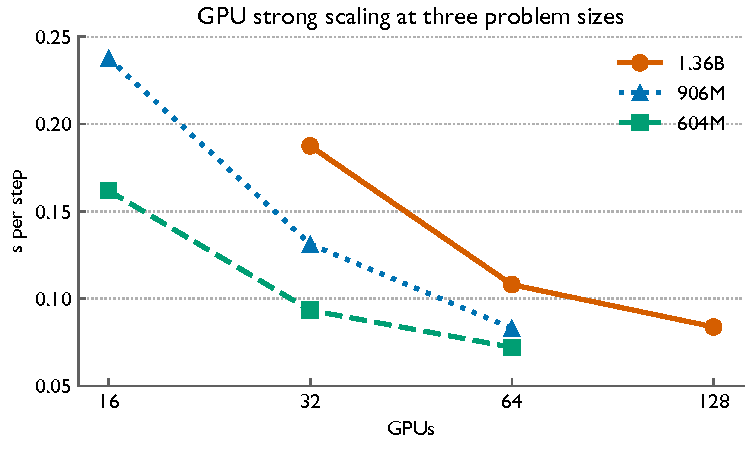
\includegraphics[width=\linewidth]{figs/fig_scaling.pdf}
\caption{Strong scaling of the wind-farm case at three problem
sizes.}
\label{fig:scaling}
\end{figure}

Figure~\ref{fig:scaling} presents strong scaling performance for the
60-turbine wind farm across vertical grid resolutions of 384, 768, and
1152 levels. The solver maintains 95\% parallel efficiency from 16 to
32 GPUs on the 472M-cell grid, 90\% on the 906M-cell grid, and 87\%
from 32 to 64 GPUs on the 1.36B-cell grid, reducing step time from
0.188\,s to 0.108\,s. Scaling extends up to 128 GPUs at 0.084\,s per time
step, achieving a throughput of 16.2 billion cell updates per second.

\begin{figure}[h]
\centering
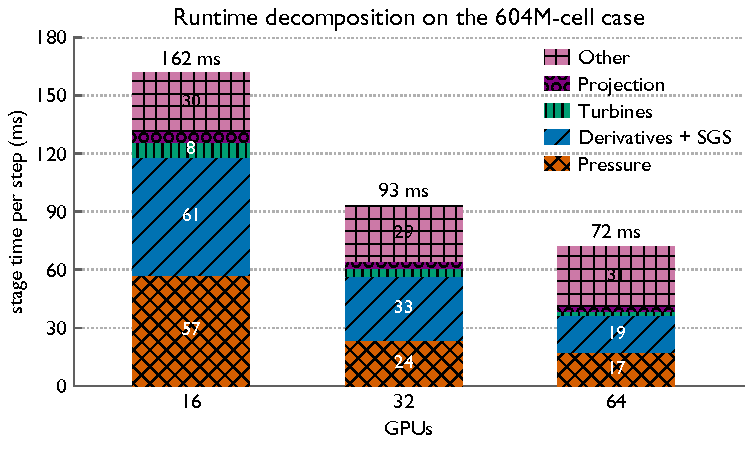
\includegraphics[width=\linewidth]{figs/fig_stagescale.pdf}
\caption{Decomposition of GPU LESGO runtime for the strong scaling cases.}
\label{fig:stagescale}
\end{figure}

To analyze scaling behavior, Figure~\ref{fig:stagescale} decomposes
runtime into individual solver stages from Algorithm~\ref{alg:step}. Each
GPU stage scales predictably with per-device workload. From 16 to 64
GPUs, SGS execution time decreases from 33\,ms to 9\,ms, derivative
evaluation drops from 24\,ms to 6\,ms, and the pressure solver exhibits
superlinear scaling up to 32 GPUs as thinner slab dimensions deepen the
tridiagonal pipeline (Section~\ref{sec:opt-tridag}). At high GPU
counts, execution time is bounded by a constant overhead of
approximately 50\,ms across 64 to 128 GPUs. This overhead primarily
stems from the \texttt{Other} stage, which includes latency-bound collectives such
as global CFL reductions to handle turbine-forcing load imbalances,
along with a constant kernel launch budget measuring 31\,ms across all
runs. The remaining overhead reflects the minimal latency floor of the
tridiagonal pipeline.

Overall step time thus follows a model composed of scalable GPU compute
and a fixed latency term. Maintaining roughly 20 million grid cells
per GPU ensures that scalable computation dominates total execution,
preserving high parallel efficiency. Consequently, parallel efficiency
at a fixed GPU count increases with problem size, directly benefiting
production-scale simulations. This fixed latency term represents an
essential algorithmic baseline. Global CFL reductions enforce adaptive
time stepping correctness, mandatory kernel dispatches persist after
batching thousands of small launches (Section~\ref{sec:opt-atm} and
Section~\ref{sec:opt-lasd}), and the pipeline latency floor represents
the physical limit of serial vertical operations (Section~\ref{sec:opt-tridag}).
Because computational kernels operate near peak DRAM bandwidth
(Fig.~\ref{fig:sol}), remaining overheads are governed by hardware
interconnect and host runtime latencies.

\begin{figure}[h]
\centering
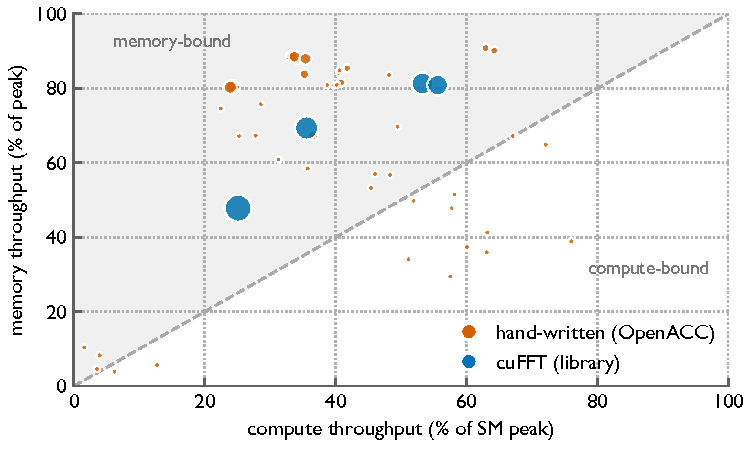
\includegraphics[width=\linewidth]{figs/fig_sol.pdf}
\caption{Nsight Compute speed-of-light utilization of every kernel in
one production step (16$\times$A100, rank 0). Point area is
proportional to each kernel's share of profiled time.}
\label{fig:sol}
\end{figure}

Nsight Compute profiling demonstrates that every major kernel
operates near the hardware's memory-bandwidth roof
(Fig.~\ref{fig:sol}). Custom field kernels achieve 67--88\% of peak DRAM
bandwidth at 24--37\% of peak compute throughput, while batched cuFFT
kernels reach 48--81\% of peak memory bandwidth. As expected for
pseudo-spectral methods, overall performance is governed by GPU memory
bandwidth.

\begin{figure}[h]
\centering
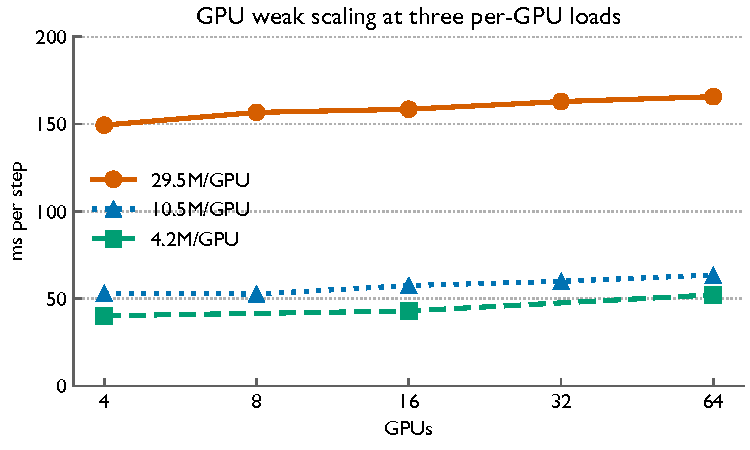
\includegraphics[width=\linewidth]{figs/fig_scaling_weak.pdf}
\caption{Weak scaling ($256\times256\times64$ points per GPU).}
\label{fig:weakscaling}
\end{figure}

Weak scaling benchmarks on the reference setup (Fig.~\ref{fig:weakscaling},
fixed at $256\times256\times64$ grid points per GPU) demonstrate 83\%
parallel efficiency up to 32 GPUs (increasing from 39.5\,ms to 47.8\,ms
per step) and 72\% efficiency at 64 GPUs (54.8\,ms per step). Stage
profiling indicates that derivative evaluation, SGS modeling, and
convection runtimes remain constant within 1\%, while pressure solve
time increases moderately due to tridiagonal chain extension across
deeper slab stacks. The 1D slab decomposition keeps all FFT transforms
rank-local, avoiding all-to-all communication overheads.

While a 2D pencil decomposition could extend rank limits further, the
1D slab structure fully satisfies our target physics. LESGO does not
pursue ever-larger wind-farm domains. It instead resolves the
turbulence physics of horizontally periodic atmospheric boundary
layers and their interaction with turbine arrays, where the grid is
set by the scales of turbulent motion rather than by domain extent.
The demonstrated range (1.36 billion cells at 87\% parallel
efficiency across 128 GPUs) therefore provides ample computational
support for production research of this class. For this reason, 
retaining the 1D slab
decomposition avoids an unnecessary architectural rewrite while
preserving structural alignment with the community-maintained CPU
codebase.

\subsection{Portability and capacity}
\label{sec:results-portability}

\begin{table}[h]
\centering
\caption{Cross-hardware behavior of the production case (no retuning).
A100 rows are Perlmutter, and H200 rows are NCSA Delta.}
\label{tab:portability}
\footnotesize
\begin{tabular}{@{}lrrl@{}}
\toprule
GPU & s/step & Mcell/s/GPU \\
\midrule
16$\times$A100 & 0.157 & 188 \\
8$\times$H200  & 0.250 & 236 \\
\bottomrule
\end{tabular}
\end{table}

Table~\ref{tab:portability} evaluates solver portability across GPU
hardware architectures without code retuning. Device memory capacity
serves as the primary portability metric for pseudo-spectral workloads.
The 472M-cell production case requires 16 A100 GPUs, whereas eight
141\,GB H200 GPUs execute the same simulation with half the GPU count.
Furthermore, H200 GPUs deliver a 26\% higher per-device throughput
(236 versus 188 million cell updates per second per GPU) because
halving the rank count doubles slab thickness and reduces inter-rank halo
and pipeline communication. Consequently, GPU memory capacity directly
enhances both simulation scale and computational efficiency in
slab-decomposed spectral solvers.

\subsection{Time to science}
\label{sec:results-science}
\fix{add science results here}

\begin{figure}[h]
\centering
\figplaceholder{figure from the production science run}
\caption{production simulation. }
\label{fig:wake}
\end{figure}
